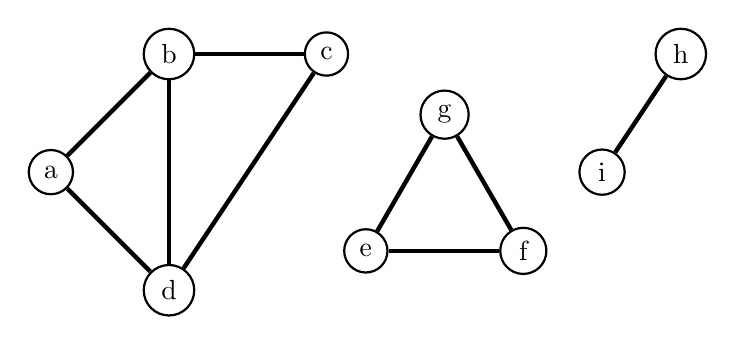
\begin{tikzpicture}
  \tikzset{vertex/.style = {draw, circle, thick}}
  \tikzset{arc/.style = {ultra thick}}
  % Component 1
  \node[vertex] (1) at (0, 1.5) {a};
  \node[vertex] (2) at (1.5, 3) {b};
  \node[vertex] (3) at (3.5, 3) {c};
  \node[vertex] (4) at (1.5, 0) {d};
  \draw[arc] (1) edge (2);
  \draw[arc] (1) edge (4);
  \draw[arc] (2) edge (3);
  \draw[arc] (2) edge (4);
  \draw[arc] (3) edge (4);
  % work in progress
  % \draw[blue, dashed, rounded corners = 8pt] (1) -- (2) -- (3) -- (4) -- (1);
  % Component 2
  \node[vertex] (5) at (4, 0.5) {e};
  \node[vertex] (6) at (6, 0.5) {f};
  \node[vertex] (7) at (5, 2.23) {g};
  \draw[arc] (5) edge (6);
  \draw[arc] (5) edge (7);
  \draw[arc] (6) edge (7);
  % Component 3
  \node[vertex] (8) at (8, 3) {h};
  \node[vertex] (9) at (7, 1.5) {i};
  \draw[arc] (8) edge (9);
\end{tikzpicture}
